%%%%%%%%%%%%%%%%%%%%%%%%%%%%%%%%%%%%%%%%%%%%%%%%%%%%%%%%%%%%%%%%%%%%
%% I, the copyright holder of this work, release this work into the
%% public domain. This applies worldwide. In some countries this may
%% not be legally possible; if so: I grant anyone the right to use
%% this work for any purpose, without any conditions, unless such
%% conditions are required by law.
%%%%%%%%%%%%%%%%%%%%%%%%%%%%%%%%%%%%%%%%%%%%%%%%%%%%%%%%%%%%%%%%%%%%

\documentclass{beamer}
\usetheme[faculty=ped,basePath=../fibeamer,logo=../fibeamer/logo/mu/Logo-UC-3.png]{fibeamer}
\graphicspath{{../resources/}}

\usepackage{algorithm}
\usepackage{algpseudocode}

\usetheme[faculty=ped]{fibeamer}
\usepackage[utf8]{inputenc}
\usepackage[
  main=english, %% By using `czech` or `slovak` as the main locale
                %% instead of `english`, you can typeset the
                %% presentation in either Czech or Slovak,
                %% respectively.
  czech, slovak %% The additional keys allow foreign texts to be
]{babel}        %% typeset as follows:
%%
%%   \begin{otherlanguage}{czech}   ... \end{otherlanguage}
%%   \begin{otherlanguage}{slovak}  ... \end{otherlanguage}
%%
%% These macros specify information about the presentation
\title{Diagrama de flujo: for, while} %% that will be typeset on the
\subtitle{Semestre II-2026} %% title page.
\author{Profesora: Andreina Cota Vidaurre}
%% These additional packages are used within the document:
\usepackage{ragged2e}  % `\justifying` text
\usepackage{booktabs}  % Tables
\usepackage{tabularx}
\usepackage{tikz}      % Diagrams
\usetikzlibrary{calc, shapes, backgrounds}
\usetikzlibrary{positioning, arrows.meta, shadows.blur, shapes.geometric}
\usepackage{amsmath, amssymb}
\usepackage{url}       % `\url`s
\usepackage{listings}  % Code listings
\usepackage{graphicx}
\usepackage{amsmath}
\usepackage[T1]{fontenc}
\usepackage{xcolor}
\usepackage{minted}
% \usepackage{adjustbox}


% Definicion de pseudocodigo en espaniol
\lstdefinelanguage{PseudocodigoES}{
    morekeywords={INICIO,FIN,PARA,HACER,SI,ENTONCES,FIN_SI,FIN_PARA,IMPRIMIR},
    sensitive=true,
    morecomment=[l]{//},
    morestring=[b]"
}

% Definicion de pseudocodigo en ingles
\lstdefinelanguage{PseudocodeEN}{
    morekeywords={BEGIN,END,FOR,DO,IF,THEN,END_IF,END_FOR,PRINT},
    sensitive=true,
    morecomment=[l]{//},
    morestring=[b]"
}

\lstset{
    basicstyle=\ttfamily\small,
    keywordstyle=\bfseries,
    columns=fullflexible,
    keepspaces=true,
    showstringspaces=false,
    frame=single,
    xleftmargin=0em,
    framexleftmargin=0em,
    framesep=2pt,
    gobble=4,
    resetmargins=true,
    aboveskip=0pt,
    belowskip=0pt
}

\lstdefinestyle{pythonstyle}{
    language=Python,
    basicstyle=\ttfamily\small,
    keywordstyle=\bfseries,
    commentstyle=\itshape,
    stringstyle=\ttfamily,
    showstringspaces=false,
    columns=fullflexible,
    keepspaces=true,
    frame=single,
    breaklines=true,
    xleftmargin=0em,
    framexleftmargin=0em,
    framesep=2pt,
    aboveskip=0pt,
    belowskip=0pt,
    gobble=4,
    resetmargins=true,
    emph={print,input,int,float,str,bool,len,range},
    emphstyle=\bfseries
}

\lstset{style=pythonstyle}

% Estilos del diagrama
% \tikzstyle{iniciofin} = [
%     ellipse,
%     minimum width=2.5cm,
%     minimum height=1cm,
%     text centered,
%     draw=black,
%     fill=blue!25
% ]

% \tikzstyle{proceso} = [
%     rectangle,
%     rounded corners,
%     minimum width=3cm,
%     minimum height=1cm,
%     text centered,
%     draw=black,
%     fill=cyan!20
% ]

% \tikzstyle{decision} = [
%     diamond,
%     aspect=2,
%     text centered,
%     draw=black,
%     fill=yellow!35
% ]

% \tikzstyle{flecha} = [
%     thick,
%     ->,
%     >=Stealth
% ]

\tikzstyle{startstop} = [
rectangle,
rounded corners,
minimum width=2.8cm,
minimum height=0.9cm,
draw
]

\tikzstyle{process} = [
rectangle,
minimum width=3cm,
minimum height=0.9cm,
draw
]

\tikzstyle{decision} = [
diamond,
aspect=2,
draw
]

\tikzstyle{arrow}=[->,>=Stealth]
% \definecolor{green_python}{HTML}{52A736}

% \newcolumntype{Y}{>{\raggedright\arraybackslash}X}

\frenchspacing
\begin{document}
  \shorthandoff{-}
  \frame[c]{\maketitle}

% \begin{darkframes}

    \begin{frame}[fragile, t]{Diagrama de flujo de \mintinline{python}{for}}
        \centering

        \begin{tikzpicture}[node distance=1.5cm]
        
        \node (start) [startstop] {Inicio};
        
        \node (init) [process, below of=start]
        {Inicializar contador};
        
        \node (cond) [decision, below of=init,yshift=-0.4cm]
        {¿Quedan elementos?};
        
        \node (body) [process, below of=cond,yshift=-0.5cm]
        {Ejecutar bloque};
        
        \node (inc) [process, below of=body]
        {Siguiente iteración};
        
        \node (end) [startstop,right=2.8cm of cond]
        {Fin};
        
        \draw [arrow] (start)--(init);
        
        \draw [arrow] (init)--(cond);
        
        \draw [arrow] (cond)--node[right]{Si}(body);
        
        \draw [arrow] (body)--(inc);
        
        \draw [arrow] (inc.west) -- ++(-1.4,0) |- (cond.west);
        
        \draw [arrow] (cond)--node[above]{No}(end);
        
        \end{tikzpicture}
    \end{frame}

    \begin{frame}{Diagrama de flujo de \mintinline{python}{for + if}}
        \begin{figure}
            \centering
            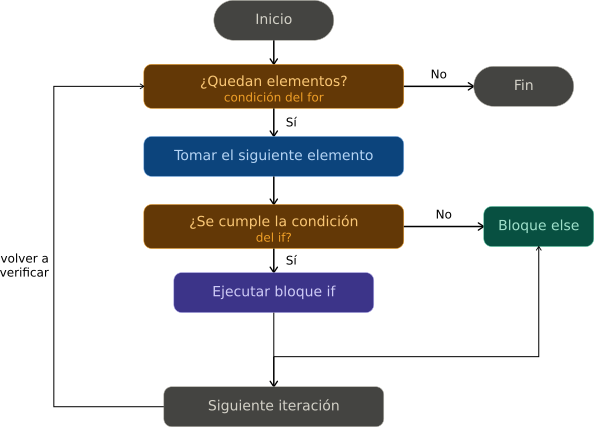
\includegraphics[width=0.9\linewidth]{flujo_for_if.png}
        \end{figure}
    \end{frame}

    \begin{frame}[fragile, t]{Control de flujo para \mintinline{python}{while}}
        \centering
        \begin{tikzpicture}[node distance=1.6cm]
        
        \node(start)[startstop]
        {Inicio};
        
        \node(cond)[decision, below of=start,yshift=-0.7cm]
        {¿Condicion verdadera?};
        
        \node(body)[process, below of=cond,yshift=-0.8cm]
        {Ejecutar bloque};
        
        \node(update)[process, below of=body]
        {Actualizar variable};
        
        \node(end)[startstop,right=2.8cm of cond]
        {Fin};
        
        \draw[arrow] (start)--(cond);
        
        \draw[arrow] (cond)--node[left]{Si}(body);
        
        \draw[arrow] (body)--(update);

        \draw [arrow] (update.west) -- ++(-1.4,0) |- (cond.west);
        
        \draw[arrow]
        (cond)--node[above]{No}(end);
        
        \end{tikzpicture}
    \end{frame}

    \begin{frame}{Diagrama de flujo de \mintinline{python}{while + if}}
        \begin{figure}
            \centering
            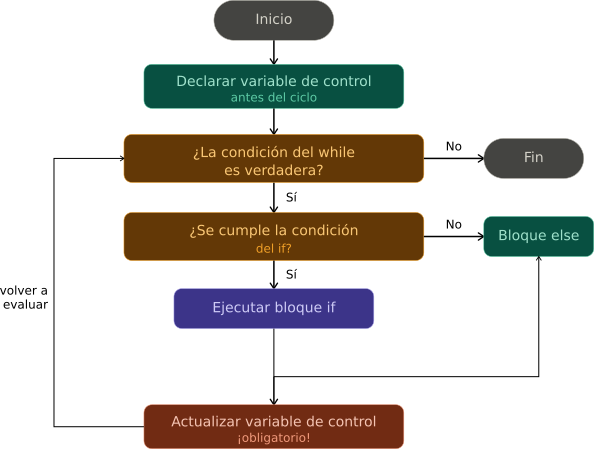
\includegraphics[width=0.8\linewidth]{flujo_while_if_1.png}
        \end{figure}
    \end{frame}

\end{document}
